%-------------------------------------------------------------------------------
%   Haskellerのための圏論
%   Keichi
%   圏論の勉強成果の個人的なまとめ
%-------------------------------------------------------------------------------

%-------------------------------------------------------------------------------
\newpage

\section{自然変換}
\subsection{定義}
$C, D$を圏とし、$\Phi,\Psi:C\to D$を関手、$X,Y\in Ob(C)$とし、
$f\in hom_C(X,Y)$とする。

\begin{figure}[htbp]
    \centering
    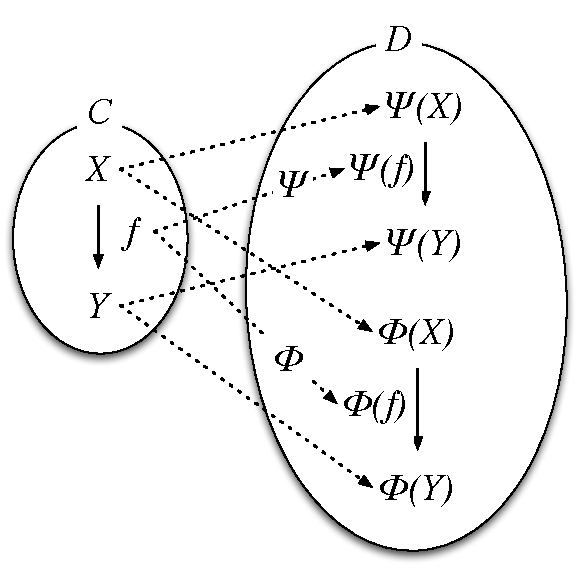
\includegraphics{diag_nt.pdf}
    \caption{関手$\Phi$と$\Psi$}
\end{figure}

自然変換(Natural Transoformation)$\eta:\Phi\to\Psi$は、$C$の各対象を、
以下の条件を満たす$D$の射と対応づける関数である。
\begin{itemize}
    \item $\forall A\in Ob(C)\to \eta_A\in hom_D(\Phi(A),\Psi(A))$
    \item $\eta_Y\circ \Phi(f)=\Psi(f)\circ\eta_X$
\end{itemize}
ここで、$\eta_A$を$A$における$\eta$のコンポーネントとよぶ。
よって、\textbf{$D$において}図\ref{figNatTrans}の関係が成り立つ。

\newpage

\begin{figure}[htbp]
    \centering
    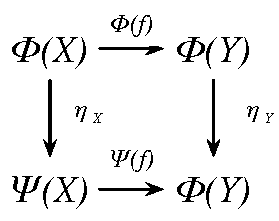
\includegraphics{diag_nt2.pdf}
    \caption{自然変換$\eta$}
    \label{figNatTrans}
\end{figure}

\subsection{Haskellによる例}
これは、図\ref{figNatTrans}関係の具体的な例Haskellで書いたものである。
\begin{lstlisting}
    --この関数はData.Maybeで定義されています。
    maybeToList :: Maybe a -> [a]
    maybeToList Nothing     =   []
    maybeToList (Just a)    =   [a]

    main = do
        print $ fmap even $ maybeToList $ Just 5
        print $ maybeToList $ fmap even $ Just 5
\end{lstlisting}
この例と上の図\ref{figNatTrans}の対応関係を考えてみる。
ファンクタ$\Psi$はList、ファンクタ$\Phi$はMaybeと対応する。
また、自然変換$\eta_X$、$\eta_Y$はmaybeToListに相当する。
(ここでmaybeToListは多相関数であるため、$\eta_X$と$\eta_Y$は
1つの多相関数maybeToListに集約される)また、$f$はevenであり
、これがfmapによってそれぞれ$\Psi(f)$と$\Phi(f)$にリフトされる。
fmapは多相であるため、$\Phi$、$\Psi$両方のファンクタの射部分に対応する。

